As engraved on his very tombstone, the configurational entropy of a system is described by Boltzmann as $k_{B} \ln W$, where $W$ is the number of available states in the system.
Considering perfectly pure Fe, in which all the Fe atoms are indistinguishable, there is exactly one state and, sensibly, zero configurational entropy.
For the perfectly pure \BTWO phase and \DOTHREE phase there are two and four unique states, respectively, due to symmetrically equivalent choices for the Al sublattice.
However, since these entropies are \emph{intrinsic}, unlike the extrinsic potential energy difference, they are immaterial for determining phase stability.
In contrast, the entropy of mixing for an ideal binary alloy is an \emph{extrinsic} property which has -- under Sterling's approximation for factorials -- a per-atom value of
%
\begin{equation}
    \label{eq:mixing}
    \Delta S_{\mathrm{mix}} = -k_B \left(c_1 \ln c_1 + c_2 \ln c_2 \right),
\end{equation}
%
where $c_1 + c_2 = 1$ are the fractional atomic composition of species 1 and 2.
Thus, in the simple approximation where vibrational entropy and thermal expansion are ignored, we can write down the per-atom free energy of the solid solution phase as
%
\begin{equation}
    \label{eq:ss_simple}
    G_{\solid} = \epsilon_\solid(c_\Al^\solid, T=0) -k_B T \left( (1-c_\Al^\solid)\ln(1 - c_\Al^\solid) + c_\Al^\solid\ln c_\Al^\solid \right),
\end{equation}
%
where $\epsilon_\solid(c_\Al^\solid, T=0)$ is just the per-atom average of the 0K minimized potential energy of a random FeAl solid solution with the Al concentration $c_\Al^\solid$.
By further making the assumption that the Al atoms are non-interacting, we can simplify this to
\begin{equation}
    \label{eq:ss_super_simple}
    G_{\solid} = \epsilon_\Fe + c_\Al^\solid \epsilon_\form -k_B T \left( (1-c_\Al^\solid)\ln(1 - c_\Al^\solid) + c_\Al^\solid\ln c_\Al^\solid \right),
\end{equation}
%
where $\epsilon_\Fe$ is the pure bulk energy and $\epsilon_\form = (E_\dilute - E_\Fe) / N$ is the difference between a supercell of $N$ atoms with one Al and a pure-Fe supercell, normalized by the number of atoms.

At equilibrium the chemical potential for all three phases must be equal, and so we can compute this value using $G_\solid$.
Conventionally we would calculate the chemical potential for each component, i.e. $\mu_\Al = \partial G / \partial N_\Al$,
but we can make a change of variable into concentration space to directly compute the chemical potential difference between Fe and Al, i.e. the cost of converting a Fe atom in the solid solution into an Al atom:
%
\begin{equation}
    \label{eq:ss_chem_pot}
    \Delta \mu = \frac{\partial G_\solid}{\partial c_\Al^\solid} = \epsilon_\form + k_B T \ln \left(\frac{c_\Al^\solid}{1 - c_\Al^\solid} \right).
\end{equation}
%
We using this we can write the free energies for the \BTWO and \DOTHREE phases as
%
\begin{eqnarray}
    G_\btwo &= \epsilon_\btwo - (0.5 - c_\Al^\solid)\Delta \mu, \label{eq:b2_super_simple} \\
    G_\dothree &= \epsilon_\dothree - (0.25 - c_\Al^\solid)\Delta \mu, \label{eq:d03_super_simple}
\end{eqnarray}
%
where the per-atom energies of the ideal phases have the same symbolism as the bulk phase, the $X-c$ term comes from the \emph{relative} excess Al in the secondary phase compared to the host solid solution, and we pick up an additional minus sign because $\Delta \mu$ must be reversed to take Al \emph{out} of the solid solution so it can be available for this phase since the total Al available to the system is fixed by the nominal alloy composition.
For the time being we also ignore configurational entropy in the secondary phases, which is available by the creation of antisites.

Consequently, when comparing the phase stability of the solid solution (SS) with the \emph{pure} \BTWO and \DOTHREE phases, configurational entropy plays a stabilizing role only for the solid solution.
I.e., in the absence of any vibrational entropy (and in our calculations ignoring quantum effects, although this need not be the case), the free energies,$G$, of each phase are
%
\begin{eqnarray}
    G_\solid &= E_\solid(c_\Al^\solid) -k_B T \left( (1-c_\Al^\solid)\ln(1 - c_\Al^\solid) + c_\Al^\solid\ln c_\Al^\solid \right) \label{eq:conf_G_SS} \\
    G_\btwo &= E_\btwo + 0.5 \Delta \mu_\Al \label{eq:conf_G_B2} \\
    G_\dothree &= E_\dothree + 0.25 \Delta \mu_\Al,\label{eq:conf_G_D03}
\end{eqnarray}
%
Where $E$ are the 0K potential energies per atom for the phase indicated in the subscript, $c_\Al^\solid$ is the solid solution Al concentration, and $\Delta \mu_\Al$ is the chemical potential of Al relative to the Fe host.

With this in mind, ignoring vibrational entropy and antisites in the secondary phases, we can calculate the relative phase fractions, $X$, by solving
%
\begin{eqnarray}
    X_\solid &= \exp(-G_\solid / k_B T) / Z, \label{eq:ss_fraction} \\
    X_\btwo &= \exp(-G_\btwo / k_B T) / Z, \label{eq:b2_fraction} \\
    X_\dothree &= \exp(-G_\dothree / k_B T) / Z, \label{eq:d03_fraction}
\end{eqnarray}
%
where
\begin{equation}
    \label{eq:partition}
    Z = \sum_{(\solid, \btwo, \dothree)} \exp(-G_i / k_B T),
\end{equation}
%
is our approximate partition function, and subject to the constraint
\begin{equation}
    \label{eq:composition_constraint}
    c_{\Al} = c_\Al^\solid X_{\solid} + 0.5 X_{\btwo} + 0.25 X_{\dothree},
\end{equation}
where $c_\Al$ is the nominal Al composition of the alloy.
Practically, we can solve this set of equations self-consistently by passing in an initial guess for $c_\Al^\solid$ to Eqs.~\ref{eq:ss_fraction}-\ref{eq:d03_fraction}, using the phase fractions in Eq.~\ref{eq:composition_constraint} to determine the resulting $c_\Al^\solid X_{\solid}$, and passing this back to the calculation of phase fractions until convergence in all four values is reached.

Following this proceedure for the 0K energies from the potential of Mendelev \etal~\cite{mendelev2005effect} gives the values for the solid solution Al content and phase fractions as a function of temperature and nominal composition shown in Figs.~\ref{fig:conf_concentration} and \ref{fig:conf_phase_fraction} respectively.
%
\begin{figure}[h]
    \label{fig:conf_concentration}
    \centering
    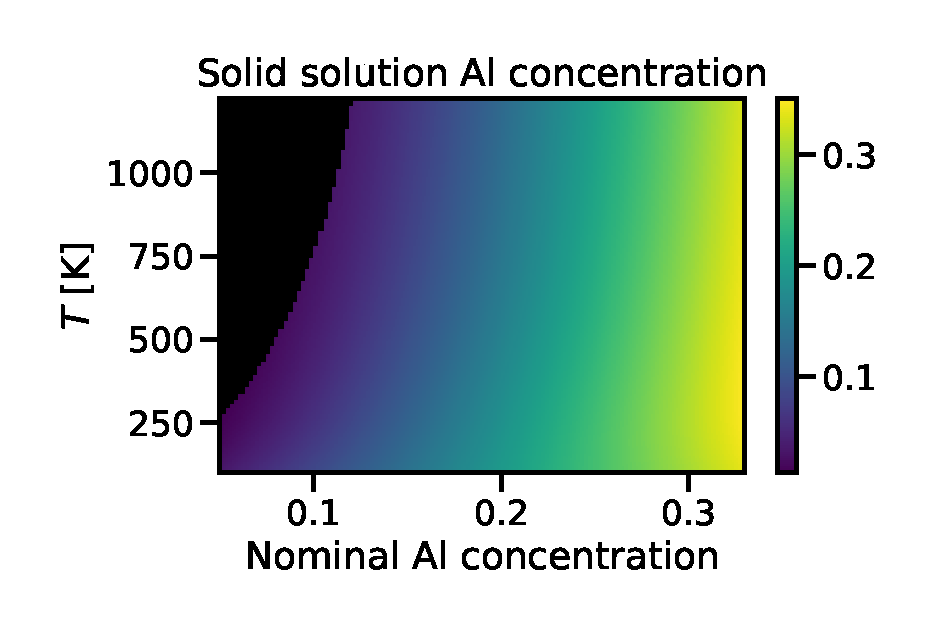
\includegraphics[width=\textwidth]{figures/conf_concentration}
    \caption{Solid solution composition in the simplified configurational-entropy-only limit, using the potential of Mendelev \etal~\cite{mendelev2005effect}. \todo{Actually, $\epsilon_\form$ is not really from the \emph{dilute} formation energy yet, but from three Al atoms in a 16-atom cell.}}
\end{figure}
%
\begin{figure}[h]
    \label{fig:conf_phase_fraction}
    \centering
    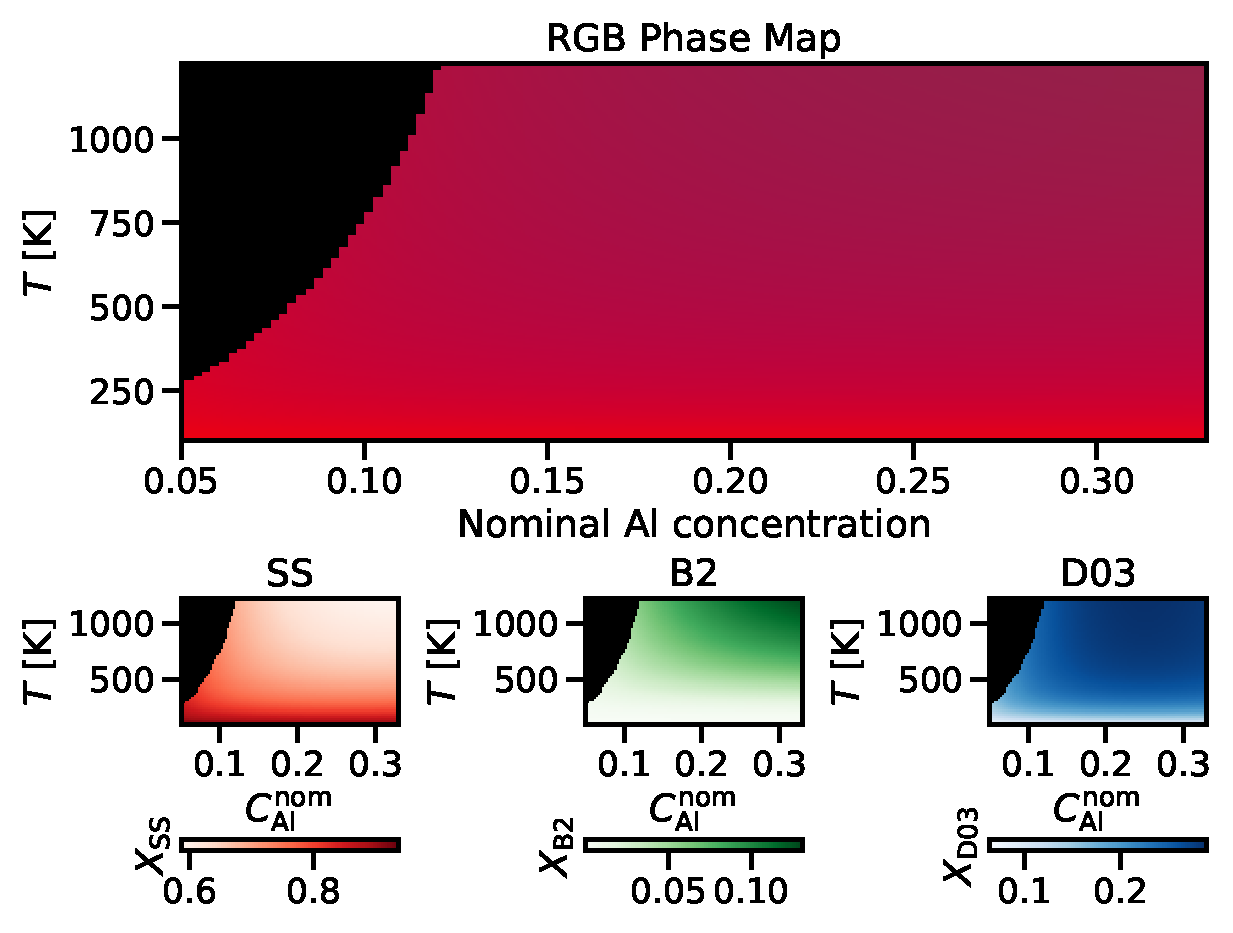
\includegraphics[width=\textwidth]{figures/conf_phase_fractions}
    \caption{Phase fractions in the simplified configurational-entropy-only limit, using the potential of Mendelev \etal~\cite{mendelev2005effect}. The main diagram shows the relative proportion of all three phases by generating an RGB-proportional color from the relative fractions, while the subplots show each phase individually. \todo{Same caveat about the source energies.}}
\end{figure}
%
We can also directly compare to the statistical results from our experimental colleagues for the nominal composition of 18\% Al they have studied, shown in Fig.~\ref{fig:conf_1d_phase_fractions}.
%
\begin{figure}[h]
    \label{fig:conf_1d_phase_fractions}
    \centering
    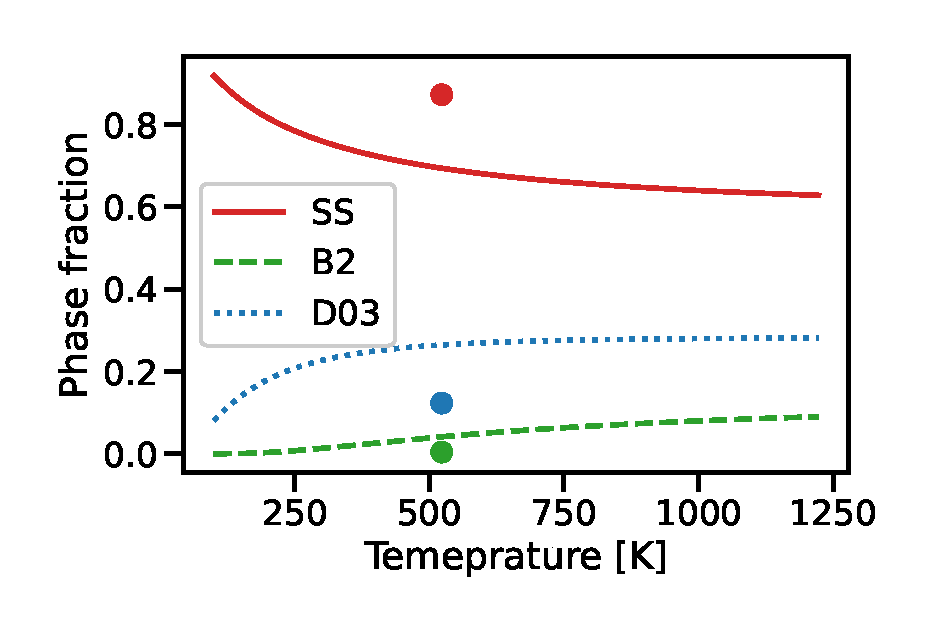
\includegraphics[width=\textwidth]{figures/conf_1d_phase_fractions}
    \caption{A slice of solid solution composition in the simplified configurational-entropy-only limit taken at the experimental alloying concentration of 18\% Al, using the potential of Mendelev \etal~\cite{mendelev2005effect}. Experiental values from annealing at 523K are shown as dots. \todo{Same caveat about the source energies.}}
\end{figure}


\subsection{Outstanding questions}
    \label{subsec:outstanding_after_simple_conf}
    \begin{itemize}
        \item How strong is the Al-Al interaction over the relevant composition domain? This can be found by calculating the expected value of $\epsilon_\solid(c_\Al^\solid)$ over a collection of random structures and comparing it to $\epsilon_\Fe + c_\Al^\solid \epsilon_\form$.
        \item What about configurational entropy in the secondary phases? In the same non-interacting limit used for the solid solution, we can calculate antisite formation energies and add antisite compositions to Eqs.~\ref{eq:b2_super_simple} and \ref{eq:d03_super_simple}. \todo{I'm not 100\% sure how the solution for phase fractions will work out with all these extra degrees of freedom yet.}
        \item What is the impact of vibrational entropy? Although computationally demanding, this can straightforwardly resolved by upgrading the 0K potential energies in Eqs.~\ref{eq:ss_super_simple}, \ref{eq:b2_super_simple} and \ref{eq:d03_super_simple} to Gibbs free energies by first calculating the Helmholtz free energy at the appropriate volumes and then using the volume-distribution method of Cheng and Ceriotti \cite{Cheng_Ceriotti_2018} to convert these to Gibbs energies. The configurational entropy remains unchanged.
        \item What about the interfacial penalties of phase coexistence, and strain effects? For this the only realistic choice is to move to full Monte Carlo/MD coupled calculations of very large cells to observe what phases actually form. This is computationally expensive and requires post-processing to identify the short range ordering, so is left until last when we are best able to assess which empirical potentials are most likely to represent the real physical system.
    \end{itemize}